\documentclass[11pt,a4paper]{article}
\usepackage[hyperref]{naaclhlt2019}
\usepackage{times}

% --- Korean translation support (xelatex + kotex) ---
\usepackage{kotex}
\usepackage{fontspec}
\setmainfont{NanumMyeongjo}[AutoFakeSlant=0.167]
\setsansfont{NanumGothic}[AutoFakeSlant=0.167]
\setmainhangulfont{NanumMyeongjo}[AutoFakeSlant=0.167]
\setsanshangulfont{NanumGothic}[AutoFakeSlant=0.167]
\setmonohangulfont{NanumGothicCoding}[AutoFakeSlant=0.167]
\setmonofont{NanumGothicCoding}[AutoFakeSlant=0.167]
\linespread{1.4}\selectfont
\renewcommand{\figurename}{그림}
\renewcommand{\tablename}{표}
\setlength{\parindent}{1.2em}
% --- end Korean support ---

\usepackage{latexsym}
\usepackage{xspace}
\usepackage{multirow}
\usepackage{url}
\usepackage{booktabs}
\usepackage{tikz,tikz-qtree}
\usepackage{pgfplots}
\usepackage{amssymb}
\usepackage{xfrac}
\usepackage{graphicx}
\usepackage{tablefootnote}
\usepackage{amsmath}
\usepackage{enumitem}
\pgfplotsset{compat=1.14}

\newcommand\BibTeX{B{\sc ib}\TeX}
\newcommand\bert{BERT\xspace}
\newcommand{\eat}[1]{\ignorespaces}


\hyphenation{OpenAI}

\definecolor{g-red}{HTML}{DB4437}
\definecolor{g-blue}{HTML}{4285F4}
\definecolor{g-green}{HTML}{0F9D58}
\definecolor{g-yellow}{HTML}{F4B400}
\definecolor{g-orange}{HTML}{FF9800}
\definecolor{g-grey}{HTML}{9E9E9E}

\setlength{\tabcolsep}{0.3em}


\newcommand\bertbase{BERT$_{\small \textsc{BASE}}$\xspace}
\newcommand\bertlarge{BERT$_{\small \textsc{LARGE}}$\xspace}

\title{\textbf{BERT}: 언어 이해를 위한 깊은 양방향 트랜스포머의 사전학습\\[2pt]\normalsize\normalfont\itshape (BERT: Pre-training of Deep Bidirectional Transformers for Language Understanding — 한국어 번역본)}

\author{Jacob Devlin \quad Ming-Wei Chang \quad Kenton Lee \quad Kristina Toutanova \\
  Google AI Language \\
  {\tt \{jacobdevlin,mingweichang,kentonl,kristout\}@google.com} \\[4pt]
  \normalfont\rmfamily 한국어 번역: Compendium (\url{https://yoon-gu.github.io/compendium/})}

\date{}

\aclfinalcopy % Uncomment this line for the final submission
\def\aclpaperid{1584} %  Enter the acl Paper ID here

% REMOVE THIS IN THE FINAL COPY!
%\hypersetup{draft}

\begin{document}
\maketitle
\begin{abstract}
  %auto-ignore
저자들은 새로운 언어 표현 모델 {\bf \bert}을 소개한다. BERT는 \textbf{B}idirectional \textbf{E}ncoder \textbf{R}epresentations from \textbf{T}ransformers의 약자다. 최근의 언어 표현 모델들~\cite{peters-etal:2018:_deep, radford-etal:2018}과 달리, \bert는 모든 층에서 좌우 양쪽 맥락을 함께 조건부로 받아 비라벨 텍스트로부터 깊은 양방향 표현을 사전학습하도록 설계되었다. 그 결과, 사전학습된 BERT 모델은 출력 층 하나만 추가해 파인튜닝하는 것만으로, 질의응답이나 언어추론 같은 폭넓은 과제에서 큰 폭의 과제별 아키텍처 수정 없이 최첨단 모델을 만들어 낼 수 있다.

\bert는 개념적으로 단순하지만 경험적으로 강력하다. 11개 자연어 처리 과제에서 새로운 최첨단 결과를 달성하며, GLUE 점수를 80.5\,\%로(절대 7.7\,\%p 개선), MultiNLI 정확도를 86.7\,\%로(절대 4.6\,\% 개선), SQuAD v1.1 질의응답 Test F1을 93.2로(절대 1.5점 개선), SQuAD v2.0 Test F1을 83.1로(절대 5.1점 개선) 끌어올렸다.


\end{abstract}

%auto-ignore
\section{서론}


언어모델 사전학습(language model pre-training)은 많은 자연어 처리(natural language processing) 과제의 성능을 끌어올리는 데 효과적임이 보여져 왔다~\cite{dai-le:2015:_semi, peters-etal:2018:_deep, radford-etal:2018, howard-ruder:2018}. 여기에는 문장 사이의 관계를 통째로 분석해 예측하는 자연어 추론(natural language inference)~\cite{bowman-etal:2015, williams-nangia-bowman:2018}과 패러프레이즈(paraphrasing)~\cite{dolan-brockett:2005:_autom} 같은 문장 수준 과제(sentence-level task), 그리고 모델이 토큰 수준의 미세한 출력을 만들어야 하는 개체명 인식(named entity recognition)과 질의응답 같은 토큰 수준 과제(token-level task)~\cite{tjong-de:2003, rajpurkar-etal:2016:_squad}가 포함된다.


사전학습된 언어 표현을 다운스트림 과제(downstream task)에 적용하는 데에는 두 가지 기존 전략이 있다 — \emph{피처 기반(feature-based)} 과 \emph{파인튜닝(fine-tuning)}. ELMo~\cite{peters-etal:2018:_deep} 같은 피처 기반 접근은, 사전학습 표현을 추가 피처(feature)로 포함하는 과제별 아키텍처(task-specific architecture)를 사용한다. Generative Pre-trained Transformer(OpenAI GPT)~\cite{radford-etal:2018} 같은 파인튜닝 접근은 과제별 파라미터(task-specific parameter)를 최소한만 추가하고, 사전학습된 \emph{모든} 파라미터를 단순히 파인튜닝하는 방식으로 다운스트림 과제에서 학습한다. 두 접근은 사전학습 단계에서 동일한 목적함수를 공유하며, 일반적인 언어 표현을 학습하기 위해 단방향(unidirectional) 언어모델을 사용한다.

저자들의 주장은, 현재 기법들이 사전학습 표현의 잠재력을 제약하고 있다는 것이다 — 특히 파인튜닝 기반 접근에서. 가장 큰 한계는 표준 언어모델이 단방향(unidirectional)이라는 점, 그리고 이로 인해 사전학습에 사용할 수 있는 아키텍처 선택이 제한된다는 점이다. 예를 들어 OpenAI GPT에서는 좌→우(left-to-right) 아키텍처를 사용하므로, 트랜스포머(Transformer)~\cite{vaswani-etal:2017:_atten}의 셀프 어텐션(self-attention) 층에서 모든 토큰(token)이 자기 이전 토큰에만 어텐션(attention)할 수 있다. 이런 제약은 문장 수준 과제에서 차선이며, 질의응답처럼 양쪽 맥락을 모두 반영해야 하는 토큰 수준 과제에 파인튜닝 기반 접근을 적용할 때는 매우 해로울 수 있다.

이 논문에서 저자들은 \bert: \textbf{B}idirectional \textbf{E}ncoder \textbf{R}epresentations from \textbf{T}ransformers를 제안하여 파인튜닝 기반 접근을 개선한다. \bert는 ``마스킹 언어모델(masked language model, MLM)''이라는 사전학습 목적함수(pre-training objective)를 사용해 앞서 언급한 단방향성 제약을 완화한다. 이 목적함수는 Cloze 과제~\cite{taylor:1953:_cloze}에서 영감을 얻었다. 마스킹 언어모델은 입력 토큰의 일부를 무작위로 마스킹(masking)하고, 마스킹된 단어의 원본 어휘 id를 그 단어의 맥락만으로 예측하는 것을 목적으로 한다. 좌→우 언어모델 사전학습과 달리, MLM 목적함수는 표현이 좌·우 맥락을 융합할 수 있게 해 주어, 깊은 양방향 트랜스포머(deep bidirectional Transformer)를 사전학습할 수 있게 한다. 마스킹 언어모델 외에, 저자들은 텍스트 쌍 표현을 함께 사전학습하는 ``다음 문장 예측(next sentence prediction, NSP)'' 과제도 사용한다. 본 논문의 기여는 다음과 같다.
\begin{itemize}[leftmargin=1em]
  \item 언어 표현 학습에서 양방향 사전학습의 중요성을 입증한다. 사전학습에 단방향 언어모델을 사용한 \citet{radford-etal:2018}과 달리, \bert는 마스킹 언어모델을 사용해 사전학습된 깊은 양방향 표현을 가능하게 한다. 또한 독립적으로 학습된 좌→우와 우→좌 LM의 얕은 결합(concatenation)을 사용한 \citet{peters-etal:2018:_deep}과도 대비된다.
  \item 사전학습된 표현이 무겁게 엔지니어링된 과제별 아키텍처의 필요성을 줄여 준다는 것을 보인다. \bert는 다수의 문장 수준 \emph{및} 토큰 수준 과제에서 최첨단 성능을 달성한 최초의 파인튜닝 기반 표현 모델이며, 많은 과제별 아키텍처를 능가한다.
  \item \bert는 11개 NLP 과제에서 최첨단을 갱신한다. 코드와 사전학습된 모델은 \url{https://github.com/google-research/bert}에서 받을 수 있다.
\end{itemize}


%auto-ignore

\section{관련 연구}
일반적인 언어 표현을 사전학습하는 시도는 오랜 역사를 갖고 있으며, 본 절에서는 가장 널리 쓰여 온 접근들을 짧게 살펴본다.


\subsection{비지도 피처 기반 접근}
폭넓게 적용 가능한 단어 표현(word representation)을 배우는 일은 수십 년 동안 활발한 연구 주제였으며, 비-신경망(non-neural) 방식~\cite{brown-etal:1992:_class, ando-zhang:2005, blitzer-mcdonald-pereira:2006:_domain}과 신경망(neural) 방식~\cite{mikolov-etal:2013, pennington-socher-manning:2014:_glove}을 모두 포함한다. 사전학습된 단어 임베딩(word embedding)은 현대 NLP 시스템의 핵심 구성요소이며, 처음부터 학습된 임베딩에 비해 큰 폭의 향상을 제공한다~\cite{turian-ratinov-bengio:2010:_word_repres}. 단어 임베딩 벡터를 사전학습하는 데에는 좌→우 언어모델링 목적함수가 사용되었고~\cite{minh09}, 좌·우 맥락에서 올바른 단어와 잘못된 단어를 구분하는 목적함수도 사용되었다~\cite{mikolov-etal:2013}.

이러한 접근은 문장 임베딩(sentence embedding)~\cite{kiros-etal:2015:_skip, logeswaran2018an}이나 단락 임베딩(paragraph embedding)~\cite{le-mikolov:2014:_distr} 같은 더 굵은 단위로도 일반화되었다. 문장 표현을 학습하기 위해 기존 연구는 후보 다음 문장의 순위를 매기는 목적함수~\cite{DBLP:journals/corr/JerniteBS17, logeswaran2018an}, 이전 문장의 표현이 주어졌을 때 다음 문장의 단어를 좌→우로 생성하는 목적함수~\cite{kiros-etal:2015:_skip}, 또는 잡음제거 오토인코더(denoising auto-encoder)에서 유도된 목적함수~\cite{hill16}를 사용해 왔다.

%
\begin{figure*}[t!]
%\small
\begin{center}
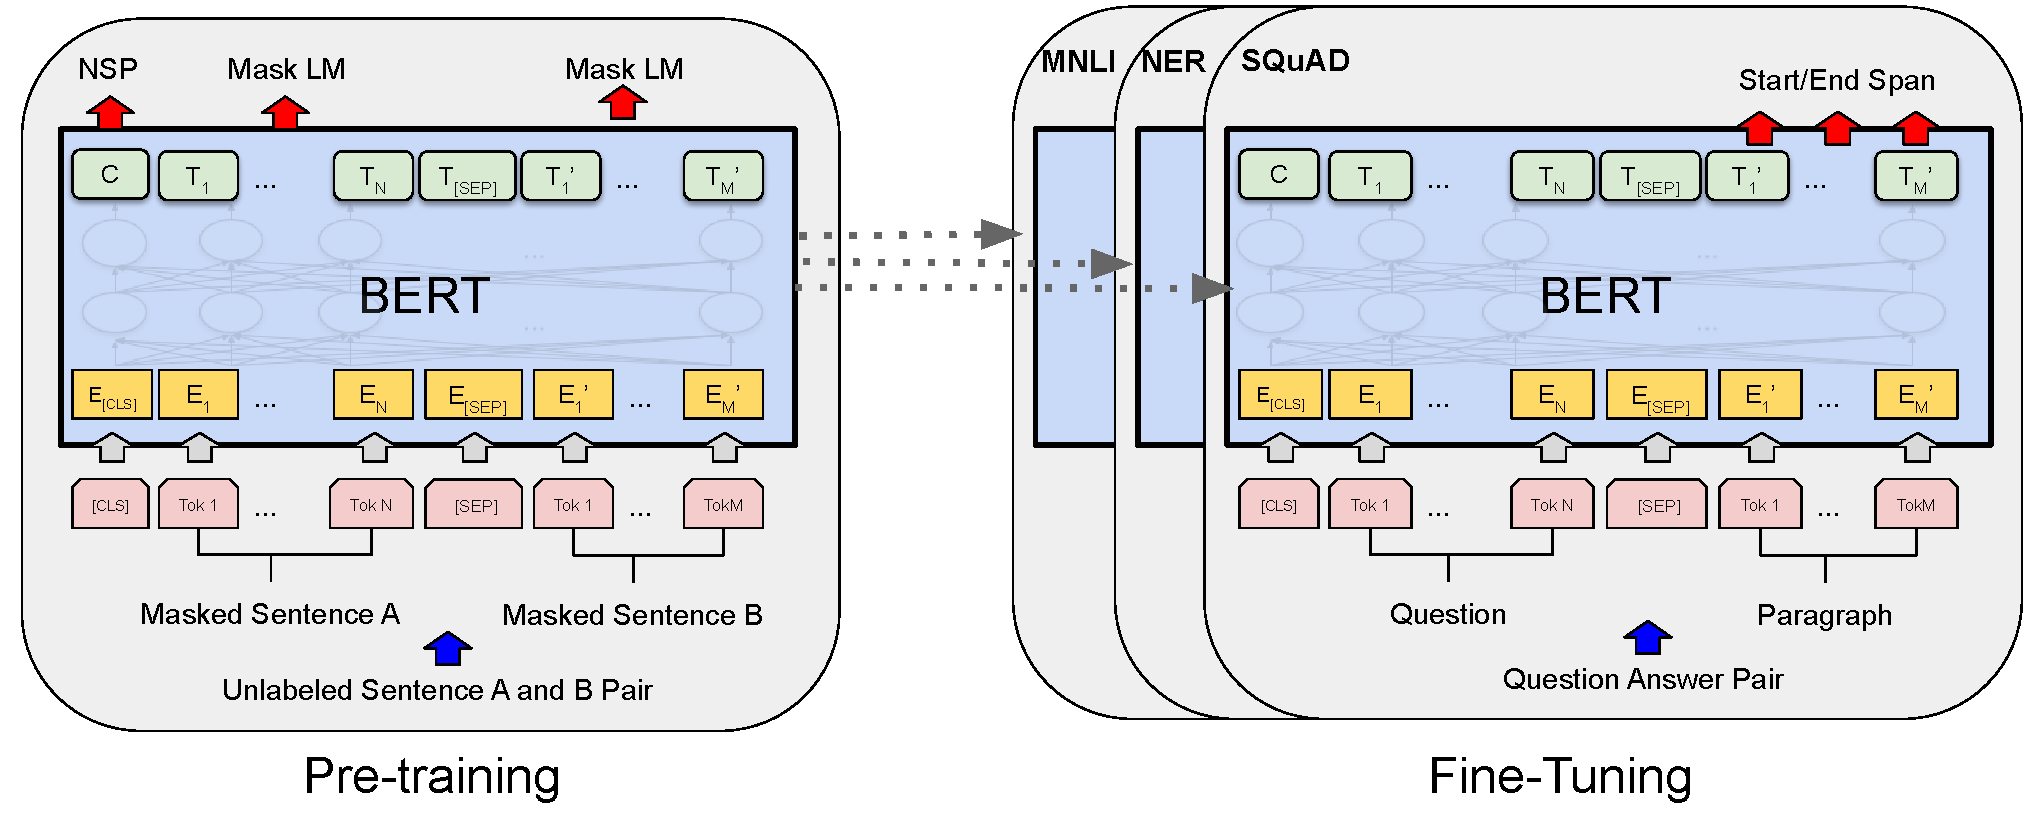
\includegraphics[width=1\textwidth]{BERT_Overall.pdf}
\end{center}
\caption{BERT의 전체 사전학습 및 파인튜닝 절차. 출력 층을 제외하면 사전학습과 파인튜닝에 동일한 아키텍처가 사용된다. 동일한 사전학습 모델 파라미터로 서로 다른 다운스트림 과제용 모델을 초기화하고, 파인튜닝 동안에는 모든 파라미터가 갱신된다. {\tt [CLS]}는 모든 입력 예시의 앞에 추가되는 특수 기호이며, {\tt [SEP]}는 특수 분리 토큰이다(예: 질문/답변 분리).}
\label{fig:bert_overall}
\end{figure*}
%



ELMo와 그 선행 연구~\cite{peters-etal:2017:_semi, peters-etal:2018:_deep}는 전통적인 단어 임베딩 연구를 또 다른 차원으로 일반화했다. 이들은 좌→우와 우→좌 언어모델로부터 \emph{맥락 민감(context-sensitive)} 피처를 추출한다. 각 토큰의 맥락 표현은 좌→우와 우→좌 표현의 결합이다. 맥락적 단어 임베딩을 기존의 과제별 아키텍처와 결합함으로써, ELMo는 질의응답~\cite{rajpurkar-etal:2016:_squad}, 감성 분석(sentiment analysis)~\cite{socher-etal:2013:_recur}, 개체명 인식~\cite{tjong-de:2003}을 포함한 여러 주요 NLP 벤치마크(benchmark)의 최첨단을 갱신했다~\cite{peters-etal:2018:_deep}.
\citet{melamud2016context2vec}은 LSTM을 이용해 좌·우 맥락 모두에서 단일 단어를 예측하는 과제를 통해 맥락 표현을 학습할 것을 제안했다. ELMo와 마찬가지로, 이 모델도 피처 기반이며 깊게 양방향이지는 않다.
\citet{fedus2018maskgan}은 cloze 과제를 텍스트 생성 모델의 견고성 향상에 활용할 수 있음을 보였다.




\subsection{비지도 파인튜닝 접근}

피처 기반 접근과 마찬가지로, 이 방향의 초기 연구도 비라벨 텍스트로부터 단어 임베딩 파라미터만 사전학습했다~\cite{collobert-weston:2008}.

더 최근에는, 맥락 토큰 표현을 만들어 내는 문장 또는 문서 인코더가 비라벨 텍스트로부터 사전학습된 뒤, 지도 학습 다운스트림 과제에 파인튜닝되어 왔다~\cite{dai-le:2015:_semi, howard-ruder:2018, radford-etal:2018}. 이 접근의 장점은 처음부터 학습해야 하는 파라미터가 적다는 점이다. 적어도 부분적으로 이 장점에 힘입어, OpenAI GPT~\cite{radford-etal:2018}는 GLUE 벤치마크~\cite{wang-etal:2018:_glue}의 많은 문장 수준 과제에서 이전의 최첨단을 달성했다. 그러한 모델의 사전학습에는 좌→우 언어모델링과 오토인코더 목적함수가 사용되어 왔다~\cite{howard-ruder:2018, radford-etal:2018,dai-le:2015:_semi}.




\subsection{지도 데이터로부터의 전이 학습}

자연어 추론~\cite{conneau-EtAl:2017:EMNLP2017}과 기계 번역(machine translation)~\cite{mccann-etal:2017:_learn_trans}처럼 데이터셋이 큰 지도 과제(supervised task)로부터의 효과적인 전이(transfer)를 보인 연구도 있다.
컴퓨터 비전(computer vision) 연구도 대규모 사전학습 모델로부터의 전이 학습(transfer learning)이 중요함을 입증해 왔으며, ImageNet으로 사전학습된 모델을 파인튜닝하는 것이 효과적인 레시피(recipe)임이 알려져 있다~\cite{imagenet_cvpr09, yosinski2014transferable}.





%auto-ignore



\section{BERT}
\label{sec:bert}

% BERT: what is pretraining and what is fine tuning at high level
본 절에서는 BERT와 그 상세 구현을 소개한다. 저자들의 프레임워크는 두 단계로 구성된다 — \emph{사전학습(pre-training)}과 \emph{파인튜닝(fine-tuning)}.
사전학습 동안 모델은 서로 다른 사전학습 과제 위에서 비라벨 데이터로 학습된다.
파인튜닝에서는 BERT 모델을 먼저 사전학습된 파라미터로 초기화한 뒤, 다운스트림 과제의 라벨 데이터를 이용해 모든 파라미터를 파인튜닝한다.
다운스트림 과제마다 별도의 파인튜닝된 모델이 만들어지지만, 모두 같은 사전학습 파라미터로 초기화된다. 그림~\ref{fig:bert_overall}의 질의응답 예시가 본 절을 관통하는 진행 예시 역할을 한다.

BERT의 두드러진 특징은 서로 다른 과제에 걸쳐 통일된 아키텍처를 사용한다는 점이다.
사전학습 아키텍처와 최종 다운스트림 아키텍처 사이에는 차이가 거의 없다.

\paragraph{모델 아키텍처}
BERT의 모델 아키텍처는 \citet{vaswani-etal:2017:_atten}에 기술되고 {\tt tensor2tensor} 라이브러리에 공개된 원본 구현에 기반한 다층 양방향 트랜스포머 인코더이다.\footnote{https://github.com/tensorflow/tensor2tensor} 트랜스포머의 사용이 일반화되었고 저자들의 구현이 원본과 거의 동일하기 때문에, 모델 아키텍처에 대한 상세 배경 설명은 생략하고 \citet{vaswani-etal:2017:_atten}이나 ``The Annotated Transformer''\footnote{http://nlp.seas.harvard.edu/2018/04/03/attention.html} 같은 훌륭한 가이드를 참고하기를 권한다.

본 연구에서, 저자들은 트랜스포머 블록의 수(즉, 층수)를 $L$, 히든 크기를 $H$, 셀프 어텐션 헤드 수를 $A$로 표기한다.\footnote{모든 경우 피드포워드/필터 크기는 $4H$로 설정한다(즉, $H=768$일 때 3072, $H=1024$일 때 4096).} 저자들은 주로 두 가지 모델 크기에 대한 결과를 보고한다 — {\bf \bertbase} ($L=12$, $H=768$, $A=12$, 총 파라미터 110M)와 {\bf \bertlarge} ($L=24$, $H=1024$, $A=16$, 총 파라미터 340M).

\bertbase는 비교 목적으로 OpenAI GPT와 같은 모델 크기를 갖도록 선택되었다. 그러나 결정적으로, BERT 트랜스포머는 양방향 셀프 어텐션을 사용하는 반면, GPT 트랜스포머는 모든 토큰이 자기 왼쪽 맥락에만 어텐션할 수 있는 제약된(셀프) 어텐션을 사용한다.\footnote{문헌에서 양방향 트랜스포머를 흔히 ``트랜스포머 인코더''라고 부르고, 좌측 맥락만 보는 버전은 텍스트 생성에 사용될 수 있어 ``트랜스포머 디코더''로 부른다는 점에 유의한다.}


\paragraph{입력/출력 표현} % Claim we shared the structures
BERT가 다양한 다운스트림 과제를 다룰 수 있게 하기 위해,
저자들의 입력 표현은 단일 문장과 한 쌍의 문장(예: $\langle$질문, 답변$\rangle$)을 모두 하나의 토큰 시퀀스 안에서 모호함 없이 표현할 수 있다. 본 연구에서 ``문장(sentence)''은 실제 언어학적 문장이 아니라 임의의 연속 텍스트 구간을 의미할 수 있다. ``시퀀스(sequence)''는 BERT의 입력 토큰 시퀀스를 가리키며, 단일 문장이거나 두 문장이 묶인 형태일 수 있다.

저자들은 30,000 토큰 어휘의 WordPiece 임베딩을 사용한다~\cite{wu-etal:2016:_googl}.
%We denote split word pieces with {\tt \#\#}. We use learned positional embeddings with supported sequence lengths up to 512 tokens.
모든 시퀀스의 첫 번째 토큰은 항상 특수 분류 토큰({\tt [CLS]})이다. 이 토큰에 해당하는 최종 은닉 상태는 분류 과제를 위한 시퀀스 전체의 집계 표현으로 사용된다.
%For non-classification tasks, this vector is ignored.
문장 쌍은 하나의 시퀀스로 묶인다. 저자들은 두 가지 방식으로 두 문장을 구분한다. 첫째, 특수 토큰({\tt [SEP]})으로 두 문장을 분리한다. 둘째, 모든 토큰에 그 토큰이 문장 {\tt A}에 속하는지 문장 {\tt B}에 속하는지를 가리키는 학습 가능한 임베딩을 더한다.
그림~\ref{fig:bert_overall}에서 보이듯, 저자들은 입력 임베딩을 $E$로, 특수 {\tt [CLS]} 토큰의 최종 은닉 벡터를 $C \in \mathbb{R}^{H}$로, $i$번째 입력 토큰의 최종 은닉 벡터를 $T_i \in \mathbb{R}^H$로 표기한다.

주어진 토큰의 입력 표현은 그에 대응하는 토큰·세그먼트·위치 임베딩을 합산해 만든다.
이 구성의 시각화는 그림~\ref{fig:input_embeddings}에서 볼 수 있다.

\begin{figure*}[ht]
\begin{center}
\hspace{-0.2in}
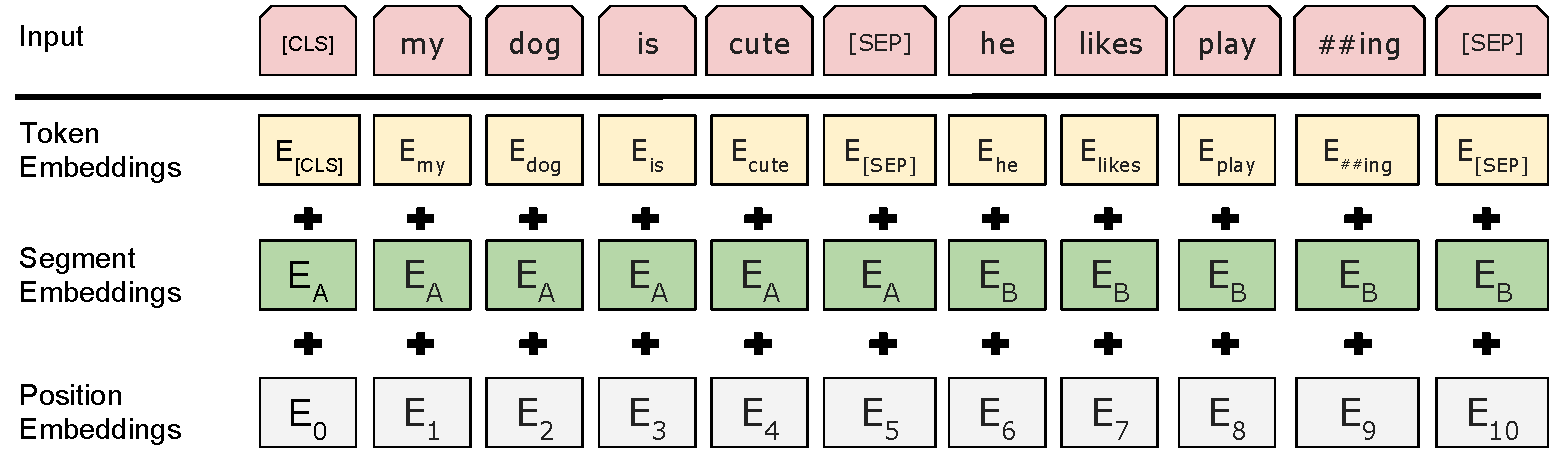
\includegraphics[width=0.85\textwidth]{Input_Emebeddings.pdf}
\end{center}
\caption{BERT 입력 표현. 입력 임베딩은 토큰 임베딩, 세그먼테이션 임베딩, 위치 임베딩의 합이다.}
\label{fig:input_embeddings}
\end{figure*}


%In the subsequent model descriptions,


\subsection{BERT 사전학습}
\label{sec:pretraining_tasks}

\citet{peters-etal:2018:_deep}이나 \citet{radford-etal:2018}과 달리, 저자들은 BERT를 사전학습할 때 전통적인 좌→우나 우→좌 언어모델을 사용하지 않는다. 대신, 본 절에서 설명하는 두 개의 비지도 과제로 BERT를 사전학습한다. 이 단계는 그림~\ref{fig:bert_overall}의 왼쪽 부분에 묘사되어 있다.

%\noindent\textbf{Task \#1: Masked LM}
\paragraph{과제 \#1: 마스킹 LM}
직관적으로, 깊은 양방향 모델이 좌→우 모델이나 좌→우/우→좌 모델의 얕은 결합보다 엄격하게 더 강력하다고 믿는 것은 합리적이다. 그러나 표준 조건부 언어모델은 좌→우 \emph{또는} 우→좌로만 학습될 수 있다 — 양방향 조건부 분포는 각 단어가 간접적으로 ``자기 자신을 보게'' 만들어, 다층 맥락에서 모델이 목표 단어를 자명하게 예측해 버리기 때문이다.

깊은 양방향 표현을 학습하기 위해, 저자들은 입력 토큰의 일정 비율을 무작위로 마스킹하고 그 마스킹된 토큰을 예측한다. 저자들은 이 절차를 ``마스킹 LM''(MLM)이라 부르며, 문헌에서는 흔히 \emph{Cloze} 과제로도 불린다~\cite{taylor:1953:_cloze}. 이 경우, 마스크 토큰에 대응하는 최종 은닉 벡터는 표준 LM처럼 어휘 위 출력 소프트맥스에 입력된다. 모든 실험에서 저자들은 각 시퀀스의 모든 WordPiece 토큰의 15\,\%를 무작위로 마스킹한다. 잡음제거 오토인코더~\cite{vincent:2008}와 달리, 입력 전체를 복원하는 대신 마스킹된 단어만 예측한다.
%Unlike \citet{melamud2016context2vec}, we mask multiple input tokens at the same time and train a deep bi-directional encoder instead of a top-level combination of left and right context encoders. In addition, we use additional token-level objectives more similar to ones in denoising auto-encoders and auto-encoders (see last two prediction tasks in the list below).

이렇게 하면 양방향 사전학습 모델을 얻을 수 있지만, 단점은 \emph{사전학습과 파인튜닝 사이의 불일치}가 생긴다는 점이다 — {\tt [MASK]} 토큰은 파인튜닝에는 등장하지 않기 때문이다. 이를 완화하기 위해, ``마스킹된'' 단어를 항상 실제 {\tt [MASK]} 토큰으로 바꾸지는 않는다. 학습 데이터 생성기는 예측 대상으로 토큰 위치의 15\,\%를 무작위로 선택한다. $i$번째 토큰이 선택되면, 80\,\% 확률로 (1) {\tt [MASK]} 토큰으로, 10\,\% 확률로 (2) 임의의 토큰으로, 10\,\% 확률로 (3) 변경 없이 원래의 $i$번째 토큰으로 둔다. 그 뒤 $T_i$가 교차 엔트로피 손실로 원본 토큰을 예측하는 데 사용된다.
이 절차의 변형들은 부록~\ref{appendix:sec:different_masks}에서 비교한다.
\vspace{.2cm}

%\noindent\textbf{Task \#2: Next Sentence Prediction (NSP)}
\paragraph{과제 \#2: 다음 문장 예측 (NSP)}
질의응답(QA)이나 자연어 추론(NLI) 같은 많은 중요한 다운스트림 과제는 두 문장 사이의 \emph{관계} 이해에 기반하는데, 이는 언어모델링이 직접 포착하지는 못한다. 문장 간 관계를 이해하는 모델을 학습하기 위해, 저자들은 어떤 단일 언어 코퍼스에서도 손쉽게 생성할 수 있는 이진화된 \emph{다음 문장 예측} 과제로 사전학습한다. 구체적으로, 각 사전학습 예시의 문장 {\tt A}와 {\tt B}를 고를 때, 50\,\% 확률로 {\tt B}는 {\tt A} 뒤에 실제로 따라오는 문장이며({\tt {\small IsNext}}로 라벨링), 50\,\% 확률로 코퍼스에서 무작위로 뽑은 문장이다({\tt {\small NotNext}}로 라벨링).
%We choose the {\tt {\small NotNext}} sentences completely at random.
그림~\ref{fig:bert_overall}에서 보이듯, $C$는 다음 문장 예측(NSP)에 사용된다.\footnote{최종 모델은 NSP에서 97\,\%--98\,\% 정확도를 달성한다.} 단순함에도 불구하고, 본 과제로 사전학습하는 것이 QA와 NLI 모두에 매우 유익함을 \S\ref{sec:task_ablation}에서 보인다.
\footnote{$C$ 벡터는 NSP로 학습된 것이므로 파인튜닝 없이는 의미 있는 문장 표현이 아니다.}
NSP 과제는 \citet{DBLP:journals/corr/JerniteBS17}과 \citet{logeswaran2018an}에서 사용된 표현 학습 목적함수와 밀접하게 관련된다. 다만 기존 연구는 문장 임베딩만 다운스트림 과제로 전이한 반면, BERT는 모든 파라미터를 전이해 최종 과제 모델 파라미터를 초기화한다.



\vspace{.3cm}
\noindent\textbf{사전학습 데이터}
사전학습 절차는 언어모델 사전학습에 관한 기존 문헌을 대체로 따른다. 사전학습 코퍼스로는 BooksCorpus(800M 단어)~\cite{zhu:2015}와 영어 Wikipedia(2,500M 단어)를 사용한다. Wikipedia에서는 본문만 추출하고 목록·표·헤더는 무시한다. Billion Word Benchmark~\cite{chelba-etal:2013:_one} 같은 문장 단위로 섞인 코퍼스가 아니라 \emph{문서 단위 코퍼스}를 사용하는 것이 결정적이다 — 그래야 길고 연속적인 시퀀스를 추출할 수 있기 때문이다.

\subsection{BERT 파인튜닝}
\label{sec:finetuning_procedure}

파인튜닝은 직관적이다. 트랜스포머의 셀프 어텐션 메커니즘은, 단일 텍스트든 텍스트 쌍이든 BERT가 입력과 출력만 적절히 교체하는 것만으로 다양한 다운스트림 과제를 모델링할 수 있게 해 주기 때문이다.
텍스트 쌍이 관여하는 응용에서 흔한 패턴은~\newcite{parikh-etal:2016, bidaf}처럼 두 텍스트를 독립적으로 인코딩한 뒤 양방향 교차 어텐션을 적용하는 것이다. BERT는 이를 셀프 어텐션 메커니즘으로 통일한다 — 두 텍스트를 이은 시퀀스를 셀프 어텐션으로 인코딩하는 것 자체가 두 문장 간의 \emph{양방향} 교차 어텐션을 효과적으로 포함하기 때문이다.


각 과제에 대해, 저자들은 과제별 입력과 출력을 단순히 BERT에 꽂아 넣고 모든 파라미터를 엔드-투-엔드로 파인튜닝한다.
%
입력 측면에서, 사전학습의 문장 {\tt A}와 문장 {\tt B}는 (1) 패러프레이즈에서의 문장 쌍, (2) 함의(entailment)에서의 가설-전제 쌍, (3) 질의응답에서의 질문-본문 쌍, (4) 텍스트 분류나 시퀀스 태깅에서의 텍스트-$\varnothing$ 퇴화 쌍에 대응된다. 출력 측면에서, 토큰 표현은 시퀀스 태깅이나 질의응답 같은 토큰 수준 과제의 출력 층에 입력되고, {\tt [CLS]} 표현은 함의나 감성 분석 같은 분류 과제의 출력 층에 입력된다.


사전학습에 비해 파인튜닝은 상대적으로 저렴하다. 본 논문의 모든 결과는 동일한 사전학습 모델에서 출발해, 단일 Cloud TPU에서 최대 1시간 안에, 또는 GPU에서 몇 시간 안에 재현할 수 있다.\footnote{예컨대, BERT SQuAD 모델은 단일 Cloud TPU에서 약 30분 만에 학습되어 Dev F1 91.0\,\%를 달성한다.}
과제별 세부 사항은 \S\ref{sec:experiments}의 해당 소절에서 기술하며, 더 자세한 내용은 부록~\ref{appendix:sec:fine_tune_details_and_figures}에서 다룬다.


\eat{The standard pattern in many NLP models is to independently encode text pairs before apply bidirectional cross attention, such as ~\newcite{parikh-etal:2016, bidaf}. BERT instead leverages the self-attention mechanism in the Transformer to unify these two stages. Encoding with self-attention is performed jointly with \emph{iterative} and \emph{bidirectional} cross attention.
Therefore, many downstream tasks---whether they involve single text or text pairs---can be modeled by simply swapping out the appropriate inputs and outputs.

At the input, sentence {\tt A} and sentence {\tt B} from pre-training are analogous to (1) sentence pairs in paraphrasing, (2) hypothesis-premise pairs in entailment, (3) question-passage pairs in question answering, and (4) a degenerate text-$\varnothing$ pair in text classification or sequence tagging. At the output, the token representations are fed into an output layer for token-level tasks, such as sequence tagging or question answering, and the {\tt [CLS]} representation is fed into an output layer for classification, such as entailment or sentiment analysis.

During the fine-tuning stage, we simply plug in the task-specific inputs and outputs into BERT and fine-tune all the parameters end-to-end. We describe the task-specific details in the corresponding subsections of Section~\ref{sec:experiments}. In-depth task specific design figures are also shown in Appendix~\ref{appendix:sec:fine_tune_details_and_figures}.
}

\eat{
\vspace{.3cm}
\noindent\textbf{Cross-attention}
BERT is designed such that it does not distinguish between self-attention used within a single sequence and cross-attention used between multiple sequences. Cross-attention between
question and passage has been shown to be important for question-answering~\cite{bidaf}, where they cross
attend question and passage for two times.
When fine-tuning a twelve-layer BERT for question answering, the question and passage will cross attend to each other for {\em twelve} times given that question and passage are packed into a single input sequence
\emph{iteratively}. Moreover, the parameters for cross-attention are pretrained. The iterative attention also happened in OpenAI GPT, but
the second sequence cannot attend to the first sequence due to the unidirectionality constraint.
}


%auto-ignore
%auto-ignore
\begin{table*}[t]
\small
\renewcommand{\arraystretch}{1.2}
\begin{center}
 \begin{tabular*}{\textwidth}{l@{\extracolsep{\fill}}cccccccc c}
    \toprule
System             &  MNLI-(m/mm)    & QQP        & QNLI       & SST-2      & CoLA       & STS-B      & MRPC       & RTE        & {\bf Average} \\
                  & 392k            & 363k       & 108k       & 67k        & 8.5k       & 5.7k       & 3.5k       & 2.5k       & -          \\ 
\hline
Pre-OpenAI SOTA    & 80.6/80.1       & 66.1       & 82.3       & 93.2       & 35.0       & 81.0       & 86.0       & 61.7       & 74.0       \\
BiLSTM+ELMo+Attn   & 76.4/76.1       & 64.8       & 79.8       & 90.4       & 36.0       & 73.3       & 84.9       & 56.8       & 71.0       \\
OpenAI GPT         & 82.1/81.4       & 70.3       & 87.4       & 91.3       & 45.4       & 80.0       & 82.3       & 56.0       & 75.1       \\

\hline
\bertbase          & 84.6/83.4       & 71.2       & 90.5       & 93.5       & 52.1       & 85.8       & 88.9       & 66.4       & 79.6       \\
\bertlarge         & {\bf 86.7/85.9} & {\bf 72.1} & {\bf 92.7} & {\bf 94.9} & {\bf 60.5} & {\bf 86.5} & {\bf 89.3} & {\bf 70.1} & {\bf 82.1} \\
    \bottomrule
   \end{tabular*}
   \caption{평가 서버({\small \url{https://gluebenchmark.com/leaderboard}})로 채점된 GLUE Test 결과. 각 과제 아래 숫자는 학습 예시 수를 의미한다. ``Average'' 열은 문제가 있는 WNLI 셋을 제외했기 때문에 공식 GLUE 점수와 약간 다르다.\footnote{\url{https://gluebenchmark.com/faq}의 질문 10 참조.}
   %OpenAI GPT = (L=12, H=768, A=12); \bertbase = (L=12, H=768, A=12); \bertlarge = (L=24, H=1024, A=16).
   BERT와 OpenAI GPT는 단일 모델·단일 과제 결과다. QQP와 MRPC는 F1, STS-B는 Spearman 상관계수, 나머지 과제는 정확도가 보고된다. BERT를 구성요소로 사용하는 엔트리는 제외했다.}
   \label{tab:glue_official}
\end{center}
\end{table*}
\footnotetext{See (10) in \url{https://gluebenchmark.com/faq}.}
\section{실험}
\label{sec:experiments}

본 절에서 저자들은 11개 NLP 과제에 대한 BERT 파인튜닝 결과를 제시한다.

\subsection{GLUE}
\label{sec:glue}

General Language Understanding Evaluation(GLUE) 벤치마크~\cite{wang-etal:2018:_glue}는 다양한 자연어 이해(natural language understanding) 과제의 모음이다.
%Most of the GLUE datasets have already existed for a number of years, but the purpose of GLUE is to (1) distribute these datasets with canonical Train, Dev, and Test splits, and (2) set up an evaluation server to mitigate issues with evaluation inconsistencies and Test set overfitting. GLUE does not distribute labels for the Test set and users must upload their predictions to the GLUE server for evaluation, with limits on the number of submissions.
GLUE 데이터셋의 상세 설명은 부록~\ref{appendix:sec:glue}에 있다.

GLUE 파인튜닝을 위해, 저자들은 \S\ref{sec:bert}에서 설명한 대로 입력 시퀀스(단일 문장 또는 문장 쌍)를 표현하고, 첫 입력 토큰({\tt [CLS]})에 해당하는 최종 은닉 벡터 $C \in \mathbb{R}^{H}$를 집계 표현으로 사용한다.
%This is demonstrated visually in Figure~\ref{fig:bert_fine_tune} (a) and (b).
파인튜닝 동안 새로 도입되는 파라미터는 분류 층 가중치(classification layer weight) $W \in \mathbb{R}^{K \times H}$뿐이며, 여기서 $K$는 라벨(label) 수다. 저자들은 $C$와 $W$로 표준 분류 손실(classification loss), 즉 $\log({\rm softmax}(CW^T))$를 계산한다.

저자들은 모든 GLUE 과제에서 배치 크기(batch size) 32, 데이터 위 3 에포크(epoch)로 파인튜닝한다. 각 과제에 대해 Dev 셋에서 가장 좋은 파인튜닝 학습률(learning rate)을 (5e-5, 4e-5, 3e-5, 2e-5 중에서) 선택한다. 또한 \bertlarge는 작은 데이터셋에서 파인튜닝이 불안정할 때가 있어, 여러 번의 무작위 재시작(random restart)을 돌리고 Dev 셋에서 가장 좋은 모델을 선택한다. 무작위 재시작에서는 동일한 사전학습 체크포인트를 쓰되, 파인튜닝 데이터 셔플과 분류 층 초기화는 다르게 한다.\footnote{GLUE 데이터셋 배포에는 Test 라벨이 포함되어 있지 않으며, 저자들은 \bertbase와 \bertlarge 각각에 대해 GLUE 평가 서버에 단 한 번씩만 제출했다.}

결과는 표~\ref{tab:glue_official}에 제시한다. \bertbase와 \bertlarge 모두 모든 과제에서 큰 차이로 모든 시스템을 능가하며, 이전 최첨단 대비 평균 정확도를 각각 4.5\,\%와 7.0\,\% 끌어올린다. \bertbase와 OpenAI GPT는 어텐션 마스킹을 제외하면 모델 아키텍처가 거의 동일하다는 점에 유의한다. 가장 크고 가장 널리 보고되는 GLUE 과제인 MNLI에서, BERT는 절대 4.6\,\% 정확도 향상을 얻는다. 공식 GLUE 리더보드\footnote{https://gluebenchmark.com/leaderboard}에서 \bertlarge는 80.5점을 얻으며, 이는 작성 시점의 OpenAI GPT 점수 72.8과 비교된다.

\bertlarge는 모든 과제에서, 특히 학습 데이터가 매우 적은 과제에서 \bertbase를 큰 폭으로 능가한다. 모델 크기의 효과는 \S\ref{sec:model_size_ablation}에서 더 자세히 다룬다.

\subsection{SQuAD v1.1}
\label{sec:squad}

Stanford Question Answering Dataset(SQuAD v1.1)은 10만 건의 크라우드소싱(crowdsourced)된 질문/답변 쌍 모음이다~\cite{rajpurkar-etal:2016:_squad}. 답을 포함하는 Wikipedia 본문과 질문이 주어졌을 때, 본문 내 답 텍스트 구간을 예측하는 과제다.

\eat{
For example:

\begin{itemize}
\item Input Question: \\{\tt {\scriptsize  Where do water droplets collide with ice crystals to form precipitation?}}
\item Input Paragraph: \\{\tt {\scriptsize  ... Precipitation forms as smaller droplets coalesce via collision with other rain drops or ice crystals within a cloud. ...}}
\item Output Answer: \\ {\tt {\scriptsize  within a cloud}}
\end{itemize}
}

그림~\ref{fig:bert_overall}에서 보이듯, 질의응답 과제에서 저자들은
입력 질문과 본문을 하나의 묶인 시퀀스로 표현하며, 질문에는 {\tt A} 임베딩을, 본문에는 {\tt B} 임베딩을 사용한다. 파인튜닝 동안 도입되는 파라미터는 시작 벡터 $S \in \mathbb{R}^H$와 종료 벡터 $E \in \mathbb{R}^H$ 두 개뿐이다.
단어 $i$가 답 구간의 시작일 확률은 $T_i$와 $S$의 내적(dot product) 뒤 본문의 모든 단어에 대해 소프트맥스를 취해 계산한다 — $P_i = \frac{e^{S{\cdot}T_i}}{\sum_j e^{S{\cdot}T_j}}$. 답 구간의 끝에도 동일한 식을 사용한다. 위치 $i$부터 $j$까지의 후보 구간 점수는 $S{\cdot}T_i + E{\cdot}T_j$로 정의되며, $j \geq i$인 구간 중 점수가 최대인 것을 예측으로 사용한다. 학습 목적함수는 올바른 시작·종료 위치의 로그우도(log-likelihood) 합이다. 학습률 5e-5, 배치 크기 32로 3 에포크 파인튜닝한다.

\input{squad_tab}


표~\ref{tab:squad_results}는 리더보드 상위 엔트리와 함께 상위 발표 시스템들의 결과를 보여 준다~\cite{bidaf,clark-gardner:2018:_simpl,peters-etal:2018:_deep,hu2017reinforced}.
SQuAD 리더보드 상위 결과들은 최신 공개 시스템 설명이 없는 경우가 있고,\footnote{QANet은 \newcite{yu-etal:2018:_qanet}에 기술되어 있으나, 게재 이후 시스템이 상당히 개선되었다.} 시스템 학습 시 어떤 공개 데이터든 사용할 수 있도록 허용된다. 그래서 저자들은 적당한 데이터 증강만을 사용한다 — TriviaQA~\cite{joshi-etal:2017:_triviaq}로 먼저 파인튜닝한 뒤 SQuAD에서 파인튜닝한다.

저자들의 가장 좋은 시스템은 앙상블(ensemble)에서 +1.5 F1, 단일 시스템에서 +1.3 F1으로 리더보드 1위 시스템을 능가한다. 사실, 저자들의 단일 BERT 모델만으로도 F1 기준 1위 앙상블 시스템을 능가한다. TriviaQA 파인튜닝 데이터를 쓰지 않으면 0.1--0.4 F1만 잃지만, 그래도 기존 시스템들을 큰 차이로 능가한다.\footnote{사용한 TriviaQA 데이터는 TriviaQA-Wiki에서 첫 400 토큰으로 구성된 단락 가운데, 제공된 가능한 답 중 적어도 하나를 포함하는 것들이다.}

\subsection{SQuAD v2.0}

SQuAD 2.0 과제는 SQuAD 1.1 문제 정의를 확장해, 제공된 단락에 짧은 답이 존재하지 않을 가능성을 허용함으로써 문제를 더 현실적으로 만든다.

저자들은 SQuAD v1.1 BERT 모델을 이 과제로 확장하기 위해 단순한 접근을 쓴다. 답이 없는 질문은 답 구간의 시작과 끝이 모두 {\tt [CLS]} 토큰인 경우로 처리한다. 시작·끝 답 구간 위치의 확률 공간을 {\tt [CLS]} 토큰의 위치까지 포함하도록 확장한다. 예측 시에는 무답 구간 점수 $s_{\tt null} = S{\cdot}C + E{\cdot}C$와 최선 비-널 구간 점수 $\hat{s_{i,j}} =  {\tt max}_{j \geq i} S{\cdot}T_i + E{\cdot}T_j$를 비교한다. $\hat{s_{i,j}} > s_{\tt null} + \tau$이면 비-널 답을 예측하며, 임계값 $\tau$는 dev 셋에서 F1을 최대화하도록 선택한다. 본 모델에는 TriviaQA 데이터를 사용하지 않았다. 학습률 5e-5, 배치 크기 48로 2 에포크 파인튜닝했다.

이전 리더보드 엔트리와 상위 발표 연구~\cite{unet,slqa}와 비교한 결과는 표~\ref{tab:squad2_results}에 있으며, 구성 요소로 BERT를 사용한 시스템은 제외했다. 이전 최고 시스템 대비 +5.1 F1 향상이 관찰된다.


\subsection{SWAG}
\label{sec:swag}
Situations With Adversarial Generations(SWAG) 데이터셋은 11.3만 건의 문장 쌍 완성(sentence-pair completion) 예시를 담고 있으며, 상식 기반 추론(grounded commonsense inference)을 평가한다~\cite{zellers2018swag}. 한 문장이 주어지면 네 개의 후보 중 가장 그럴듯한 이어지는 문장을 고르는 과제다.


SWAG 데이터셋에 대한 파인튜닝에서, 저자들은 주어진 문장(문장 {\tt A})과 가능한 이어짐(문장 {\tt B})의 결합을 각각 담은 네 개의 입력 시퀀스를 만든다. 도입되는 과제별 파라미터는 {\tt [CLS]} 토큰 표현 $C$와의 내적이 각 후보의 점수가 되는 벡터 하나뿐이며, 그 점수는 소프트맥스 층으로 정규화된다.

학습률 2e-5, 배치 크기 16으로 3 에포크 파인튜닝한다. 결과는 표~\ref{tab:swag_official}에 제시한다. \bertlarge는 저자들의 베이스라인 ESIM+ELMo 시스템을 +27.1\,\%, OpenAI GPT를 +8.3\,\% 능가한다.

%auto-ignore
\begin{table}[tb]
\begin{center}
{
\small
 \begin{tabular}{lcc}
    \toprule
System             &  Dev    & Test\\ 
\midrule
ESIM+GloVe   & 51.9       & 52.7 \\
ESIM+ELMo    & 59.1       & 59.2 \\
OpenAI GPT    & -       & 78.0 \\
\midrule
\bertbase    & 81.6       &  - \\
\bertlarge   & {\bf 86.6} & {\bf 86.3} \\
\midrule
Human (expert)$^\dagger$ & - & 85.0 \\
Human (5 annotations)$^\dagger$        & -          & 88.0 \\
\bottomrule
\end{tabular}
}
\caption{SWAG Dev·Test 정확도.
$^\dagger$사람 성능은 SWAG 논문에서 보고된 대로 100개 샘플로 측정한 값이다.}
\label{tab:swag_official}
\end{center}
\end{table}


%auto-ignore
\section{절제 연구}
\label{sec:ablation}
본 절에서 저자들은 각 요소의 상대적 중요도를 더 잘 이해하기 위해 BERT의 여러 측면에 대한 절제 실험(ablation study)을 수행한다. 추가 절제 연구는 부록~\ref{appendix:sec:more_ablation_studies}에서 확인할 수 있다.

\subsection{사전학습 과제의 효과}

\label{sec:task_ablation}
저자들은 \bertbase와 정확히 동일한 사전학습 데이터, 파인튜닝 방식, 하이퍼파라미터를 쓰면서 두 가지 사전학습 목적함수를 평가해 BERT의 깊은 양방향성의 중요성을 입증한다.
\vspace{0.3cm}
\\
\noindent\textbf{No NSP}: ``마스킹 LM''(MLM)으로 학습되지만 ``다음 문장 예측''(NSP) 과제 없이 학습되는 양방향 모델.\\
\noindent\textbf{LTR \& No NSP}: MLM이 아닌 표준 좌→우(LTR) LM으로 학습되는 좌측 맥락만 사용하는 모델. 좌측 전용 제약은 파인튜닝에도 동일하게 적용했는데, 이 제약을 제거하면 사전학습/파인튜닝 불일치가 생겨 다운스트림 성능이 떨어졌기 때문이다. 또한 이 모델은 NSP 과제 없이 사전학습된다. 이 모델은 OpenAI GPT와 직접 비교 가능하지만, 더 큰 학습 데이터셋과 본 논문의 입력 표현·파인튜닝 방식을 사용한다.
%auto-ignore
\begin{table}[t]
\small
 \begin{tabular}{@{}lccccc@{}}
    \toprule
              & \multicolumn{5}{c}{Dev 셋} \\
   과제 & MNLI-m & QNLI & MRPC & SST-2 & SQuAD     \\
         & (Acc) & (Acc) & (Acc) & (Acc) & (F1)     \\
     \midrule
\bertbase       & 84.4 & 88.4 & 86.7 & 92.7 & 88.5 \\
No NSP          & 83.9 & 84.9 & 86.5 & 92.6 & 87.9 \\
LTR \& No NSP   & 82.1 & 84.3 & 77.5 & 92.1 & 77.8 \\
\quad + BiLSTM  & 82.1 & 84.1 & 75.7 & 91.6 & 84.9 \\
     \bottomrule
   \end{tabular}
   \caption{\bertbase 아키텍처를 사용한 사전학습 과제 절제. ``No NSP''는 다음 문장 예측 과제 없이 학습된다. ``LTR \& No NSP''는 OpenAI GPT처럼 다음 문장 예측 없이 좌→우 LM으로 학습된다. ``+ BiLSTM''은 파인튜닝 시 ``LTR + No NSP'' 모델 위에 무작위 초기화된 BiLSTM을 추가한 것이다.
   }
   \label{tab:task_ablation}    
\end{table}

먼저 NSP 과제의 영향을 살핀다. 표~\ref{tab:task_ablation}에서 보이듯, NSP를 제거하면 QNLI, MNLI, SQuAD 1.1에서 성능이 크게 떨어진다. 다음으로, ``No NSP''와 ``LTR \& No NSP''를 비교해 양방향 표현 학습의 영향을 평가한다. LTR 모델은 모든 과제에서 MLM 모델보다 성능이 낮으며, MRPC와 SQuAD에서 큰 폭의 하락을 보인다.

SQuAD에서는 LTR 모델이 토큰 예측에서 좋지 않은 성능을 낼 것임이 직관적으로 분명하다 — 토큰 수준 은닉 상태에 우측 맥락이 전혀 없기 때문이다.
LTR 시스템을 강화하려는 성실한 시도로, 저자들은 그 위에 무작위로 초기화된(randomly initialized) BiLSTM을 추가했다. 이는 SQuAD 결과를 의미 있게 개선하지만, 사전학습된 양방향 모델의 결과에는 한참 못 미친다. BiLSTM은 GLUE 과제에서는 오히려 성능을 떨어뜨린다.

저자들은 ELMo처럼 별도의 LTR과 RTL 모델을 학습한 뒤 각 토큰을 두 모델의 결합으로 표현하는 것도 가능함을 인정한다. 그러나 (a) 이는 단일 양방향 모델보다 두 배 비싸고, (b) RTL 모델이 답을 질문에 조건부로 둘 수 없으므로 QA 같은 과제에는 비직관적이며, (c) 모든 층에서 좌·우 맥락을 모두 사용할 수 있는 깊은 양방향 모델보다 엄격하게 약하다.


\subsection{모델 크기의 효과}
\label{sec:model_size_ablation}

본 절에서 저자들은 모델 크기가 파인튜닝 과제 정확도에 미치는 영향을 탐구한다. 층수, 은닉 유닛 수, 어텐션 헤드 수가 다른 여러 BERT 모델을 학습했고, 그 외의 하이퍼파라미터와 학습 절차는 앞서 기술한 것과 동일하게 두었다.

선택된 GLUE 과제의 결과는 표~\ref{tab:size_ablation}에 있다. 본 표에서 저자들은 5번의 무작위 재시작 파인튜닝의 평균 Dev 셋 정확도를 보고한다. 더 큰 모델이 네 데이터셋 모두에서 엄격한 정확도 향상을 가져옴을 알 수 있다. 학습 라벨이 3,600개에 불과하고 사전학습 과제와 상당히 다른 MRPC조차도 마찬가지다. 또한 기존 문헌에 비해 이미 상당히 큰 모델 위에서 이 정도 향상을 얻을 수 있다는 점은 다소 놀라울 수 있다. 예컨대 \citet{vaswani-etal:2017:_atten}에서 탐구한 가장 큰 트랜스포머는 인코더에 100M 파라미터를 가지는 ($L=6$, $H=1024$, $A=16$)이고, 문헌에서 저자들이 발견한 가장 큰 트랜스포머는 235M 파라미터의 ($L=64$, $H=512$, $A=2$)이다~\cite{alrfou:2018}. 이에 비해 \bertbase는 110M, \bertlarge는 340M 파라미터를 갖는다.

%auto-ignore
\begin{table}[b]
\begin{center}
{\small
\begin{tabular}{@{}rrrcccc@{}}
  \toprule
  \multicolumn{3}{c}{하이퍼파라미터}      &      & \multicolumn{3}{c}{Dev 셋 정확도} \\
  \midrule
  \#L & \#H &\#A & LM (ppl) & MNLI-m & MRPC &SST-2               \\
  \midrule
  \
   3 &  768 & 12 & 5.84 & 77.9 & 79.8 & 88.4 \\
   6 &  768 &  3 & 5.24 & 80.6 & 82.2 & 90.7 \\
   6 &  768 & 12 & 4.68 & 81.9 & 84.8 & 91.3 \\
  12 &  768 & 12 & 3.99 & 84.4 & 86.7 & 92.9 \\
  12 & 1024 & 16 & 3.54 & 85.7 & 86.9 & 93.3 \\
  24 & 1024 & 16 & 3.23 & 86.6 & 87.8 & 93.7 \\
\bottomrule
\end{tabular}
} % small
\end{center}
\caption{\label{tab:size_ablation} BERT 모델 크기 절제. \#L = 층수, \#H = 은닉 크기, \#A = 어텐션 헤드 수. ``LM (ppl)''은 홀드아웃 학습 데이터의 마스킹 LM 퍼플렉시티다.}
\end{table}


기계 번역과 언어 모델링 같은 대규모 과제에서 모델 크기를 키우면 지속적인 향상이 따라온다는 점은 오래 전부터 알려져 있고, 표~\ref{tab:size_ablation}이 보여 주는 홀드아웃(held-out) 학습 데이터의 LM 퍼플렉시티(perplexity)에서도 이를 확인할 수 있다. 그러나 모델이 충분히 사전학습되었다는 전제 하에 \emph{매우 작은 규모의 과제}에서도 극단적인 모델 크기로의 스케일링이 큰 향상을 가져온다는 점을 설득력 있게 보인 것은 본 연구가 처음이라고 저자들은 본다. \citet{peters2018dissecting}은 사전학습 bi-LM의 층수를 2에서 4로 늘렸을 때 다운스트림 영향에 대해 혼합된 결과를 제시했고, \citet{melamud2016context2vec}은 은닉 차원을 200에서 600으로 늘리면 도움이 되지만 1,000으로 더 늘려도 추가 향상은 없었다고 짤막하게 언급했다. 이 두 선행 연구는 모두 피처 기반 접근을 사용했다 --- 저자들의 가설은, 모델이 다운스트림 과제 위에서 직접 파인튜닝되고 무작위 초기화된 추가 파라미터가 매우 적게만 도입될 때에는, 다운스트림 데이터가 매우 작더라도 과제별 모델이 더 크고 표현력 있는 사전학습 표현으로부터 이득을 볼 수 있다는 것이다.



\subsection{BERT의 피처 기반 접근}
\label{sec:ner}
지금까지 제시한 BERT 결과는 모두, 사전학습 모델 위에 단순한 분류 층을 더한 뒤 다운스트림 과제 위에서 모든 파라미터를 함께 파인튜닝하는 파인튜닝 접근을 사용했다. 그러나 사전학습 모델에서 고정 피처를 추출하는 피처 기반 접근에도 일정한 장점이 있다. 첫째, 모든
%NLP
과제가 트랜스포머 인코더 아키텍처로 손쉽게 표현되지는 않으며, 따라서 과제별 모델 아키텍처가 추가로 필요할 수 있다. 둘째, 학습 데이터의 비싼 표현을 한 번만 미리 계산해 두고 그 위에서 더 저렴한
%being able to
%less expensive
모델로 여러 실험을 돌릴 수 있다는 큰 계산 이점이 있다.

본 절에서 저자들은 CoNLL-2003 개체명 인식(named entity recognition, NER) 과제~\cite{tjong-de:2003}에 BERT를 적용해 두 접근을 비교한다. BERT 입력에는 대소문자를 보존하는 WordPiece 모델을 사용하며, 데이터가 제공하는 최대 문서 맥락을 함께 포함한다. 표준 관행을 따라 이를 태깅(tagging) 과제로 정식화하지만, 출력에는 CRF(Conditional Random Field) 층을 사용하지 않는다. 첫 서브토큰의 표현을 NER 라벨 집합 위 토큰 수준 분류기의 입력으로 사용한다.


파인튜닝 접근을 절제하기 위해, 저자들은 BERT의 어떤 파라미터도 파인튜닝하지 \emph{않은} 채 하나 이상의 층의 활성을 추출하는 피처 기반 접근을 적용한다. 이렇게 얻은 맥락 임베딩은, 분류 층 이전에 무작위 초기화된 두 층 768차원 BiLSTM의 입력으로 사용된다.

결과는 표~\ref{tab:pretrained_embeddings}에 제시한다. \bertlarge는 최첨단 방법들과 경쟁력 있는 성능을 보인다. 가장 좋은 방법은 사전학습 트랜스포머의 상위 네 개 은닉 층의 토큰 표현을 결합하는 것이며, 이는 모델 전체를 파인튜닝하는 결과보다 0.3 F1만 뒤진다. 이는 BERT가 파인튜닝 접근과 피처 기반 접근 양쪽 모두에 효과적임을 보여 준다.


%auto-ignore

\begin{table}[t]
\small
\centering
 \begin{tabular}{@{}lcc@{}}
\toprule
System & Dev F1 & Test F1 \\
\midrule
ELMo~\cite{peters-etal:2018:_deep}& 95.7 & 92.2 \\
CVT~\cite{clark2018semi} & - & 92.6 \\
CSE~\cite{akbik2018contextual} & - & {\bf 93.1} \\
\midrule
파인튜닝 접근 & & \\
\;\;\;\bertlarge  & 96.6 & 92.8 \\
\;\;\;\bertbase& 96.4 & 92.4 \\
\midrule
피처 기반 접근 (\bertbase) &  &  \\
\;\;\;Embeddings & 91.0 &- \\
\;\;\;Second-to-Last Hidden   & 95.6&- \\
\;\;\;Last Hidden            & 94.9&- \\
\;\;\;Weighted Sum Last Four Hidden        & 95.9&- \\
\;\;\;Concat Last Four Hidden        & 96.1&- \\
\;\;\;Weighted Sum All 12 Layers        & 95.5&- \\
\bottomrule
\end{tabular}
\caption{CoNLL-2003 개체명 인식 결과. 하이퍼파라미터는 Dev 셋을 이용해 선택했다. 보고된 Dev·Test 점수는 그 하이퍼파라미터로 5번 무작위 재시작한 결과의 평균이다.
}
\label{tab:ner_results}    
\label{tab:pretrained_embeddings}    
\end{table}


%auto-ignore
\section{결론}
언어모델을 이용한 전이 학습이 가져온 최근의 경험적 향상은, 풍부한 비지도 사전학습이 많은 언어 이해 시스템의 핵심 구성요소임을 보여 주었다. 특히 이 결과들은 자원이 적은 과제에서도 깊은 단방향 아키텍처의 이점을 누릴 수 있게 해 준다. 본 논문의 주요 기여는 이러한 발견을 깊은 \emph{양방향} 아키텍처로까지 더 일반화하여, 동일한 사전학습 모델이 폭넓은 NLP 과제를 성공적으로 처리할 수 있게 만든 것이다.


\bibliographystyle{acl_natbib}
\bibliography{lumiere}

%\clearpage
\pagenumbering{arabic} 
\appendix                                     
%auto-ignore
\begin{center}
{\bf \large{
    ``BERT: Pre-training of Deep Bidirectional Transformers for Language Understanding'' 부록}}
\end{center}


부록은 세 개의 절로 구성된다.
\begin{itemize}
   \item BERT의 추가 구현 세부 사항은 부록~\ref{appendix:sec:bert_description}에서 제시한다.

   \item 실험에 대한 추가 세부 사항은 부록~\ref{appendix:sec:exp_details}에서 제시한다.


   \item 추가 절제 연구는 부록~\ref{appendix:sec:more_ablation_studies}에서 제시한다.

   BERT에 대한 추가 절제 연구로는 다음을 다룬다.
   \begin{itemize}
      \item 학습 스텝 수의 효과
      \item 서로 다른 마스킹 절차에 대한 절제
   \end{itemize}
\end{itemize}
%auto-ignore
\section{BERT 추가 세부 사항}
\label{appendix:sec:bert_description}



\begin{figure*}[ht]
\begin{center}
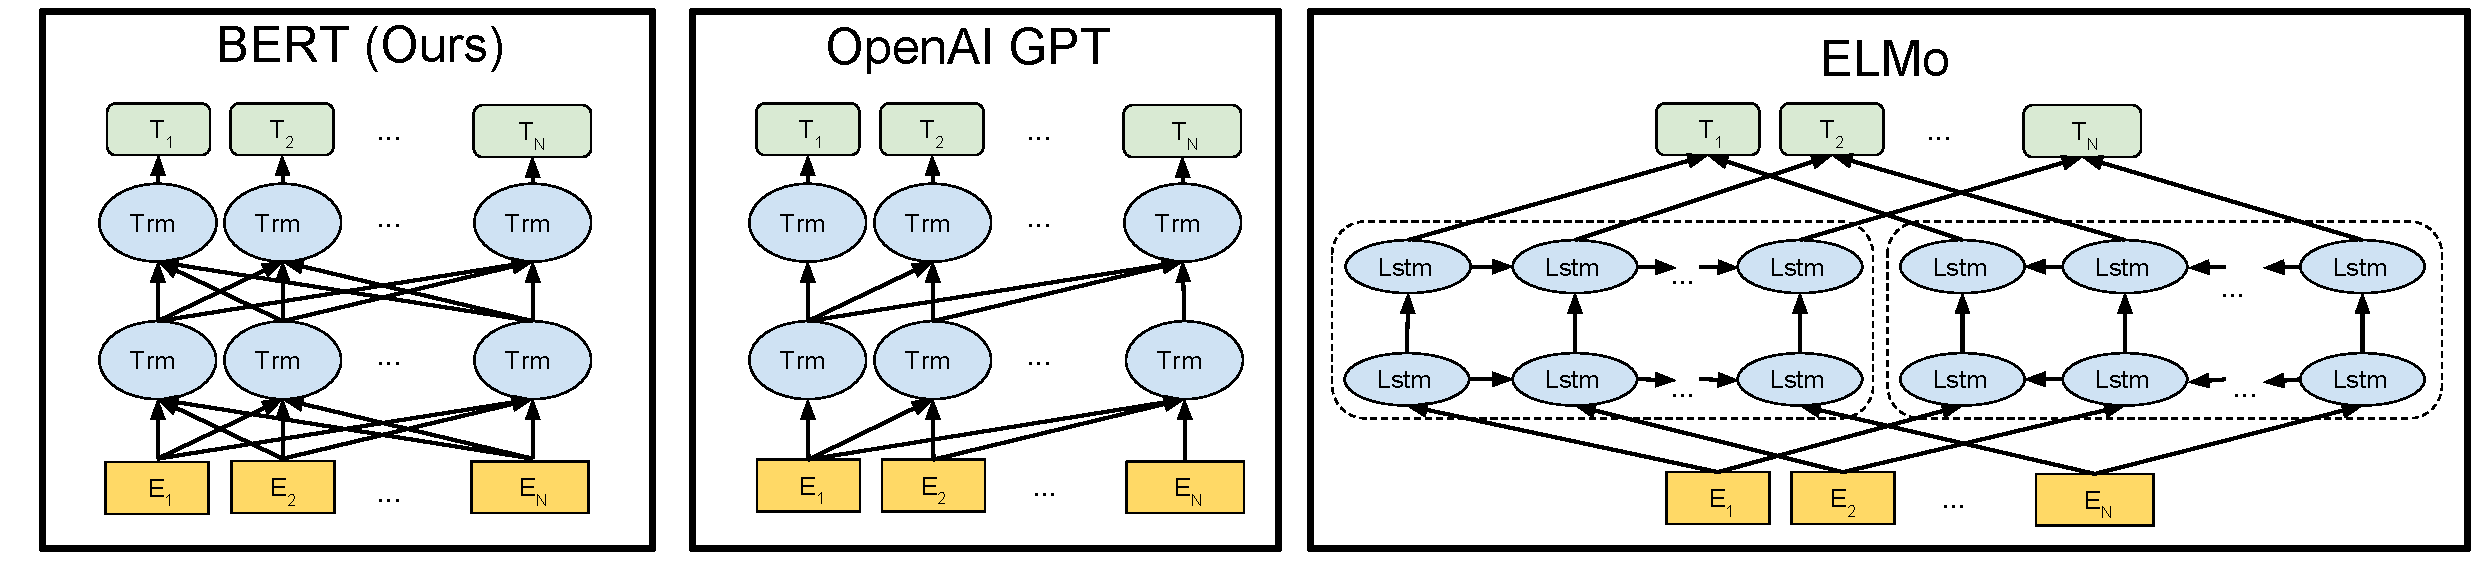
\includegraphics[width=\textwidth]{BERT_comparisons.pdf}
\end{center}
\caption{사전학습 모델 아키텍처의 차이. BERT는 양방향 트랜스포머를 사용한다. OpenAI GPT는 좌→우 트랜스포머를 사용한다. ELMo는 독립적으로 학습된 좌→우와 우→좌 LSTM의 결합을 사용해 다운스트림 과제용 피처를 생성한다. 셋 중에서, 모든 층에서 좌·우 맥락에 함께 조건화되는 표현을 만드는 것은 \bert뿐이다. 아키텍처 차이 외에, BERT와 OpenAI GPT는 파인튜닝 접근이고 ELMo는 피처 기반 접근이라는 차이도 있다.}
\label{fig:BERT_comparisons}
\end{figure*}


\subsection{사전학습 과제 예시}
다음에 사전학습 과제의 예시를 제공한다.

\paragraph{마스킹 LM과 마스킹 절차}

비라벨 문장이 {\tt {\small my dog is hairy}}이고, 무작위 마스킹 절차에서 4번째 토큰({\tt {\small hairy}}에 해당)을 선택했다고 가정하면, 마스킹 절차는 다음과 같이 더 자세히 표현될 수 있다.
\begin{itemize}
%\item Rather than {\em always} replacing the chosen words with {\tt [MASK]}, the data generator will do the following:
\item 80\,\% 확률로 단어를 {\tt [MASK]} 토큰으로 바꾼다 — 예: {\tt {\small my dog is hairy $\rightarrow$ my dog is [MASK]}}
\item 10\,\% 확률로 단어를 무작위 단어로 바꾼다 — 예: {\tt {\small my dog is hairy $\rightarrow$ my dog is apple}}
\item 10\,\% 확률로 단어를 그대로 둔다 — 예: {\tt {\small my dog is hairy $\rightarrow$ my dog is hairy}}. 그 목적은 표현이 실제 관측된 단어 쪽으로 편향되도록 만드는 것이다.
\end{itemize}

이 절차의 장점은, 트랜스포머 인코더가 어떤 단어를 예측하라고 요청받을지, 어떤 단어가 무작위 단어로 바뀌었는지를 미리 알 수 없다는 점이다. 따라서 인코더는 \emph{모든} 입력 토큰에 대한 분포적 맥락 표현을 유지하지 않을 수 없다. 또한 무작위 치환은 전체 토큰의 1.5\,\%(15\,\%의 10\,\%)에서만 일어나므로, 모델의 언어 이해 능력을 해치지는 않는 것으로 보인다. 이 절차의 영향은 \S\ref{appendix:sec:different_masks}에서 평가한다.

표준 언어모델 학습과 달리, 마스킹 LM은 각 배치에서 토큰의 15\,\%에 대해서만 예측을 수행한다. 이는 모델이 수렴하는 데 더 많은 사전학습 스텝이 필요할 수 있음을 시사한다. \S\ref{sec:num_training_steps}에서 저자들은 MLM이 모든 토큰을 예측하는 좌→우 모델보다 약간 느리게 수렴하지만, MLM의 경험적 향상이 늘어난 학습 비용을 훨씬 능가함을 보인다.

\paragraph{다음 문장 예측}

다음 문장 예측 과제는 다음 예시들로 표현될 수 있다.
\begin{align*}
\text{Input\;} &= \text{\tt {\scriptsize [CLS] the man went to [MASK] store [SEP]}} \\
& \text{\tt {\scriptsize \;\;\;\;\;\;\;he bought a gallon [MASK] milk [SEP]}}\\
\text{Label} &= \text{\tt {\scriptsize IsNext}} \\
\\
\text{Input\;} &= \text{\tt {\scriptsize [CLS] the man [MASK] to the store [SEP]}}\\
&\text{\tt {\scriptsize \;\;\;\;\;\;\;penguin [MASK] are flight \#\#less birds [SEP]}}\\
\text{Label} &= \text{\tt {\scriptsize NotNext}}
\end{align*}

\subsection{사전학습 절차}
\label{sec:pretraining_procedure}

각 학습 입력 시퀀스를 만들기 위해, 저자들은 코퍼스에서 두 개의 텍스트 구간을 샘플링한다 — 보통 단일 문장보다 훨씬 길지만(때로는 더 짧을 수도 있음) ``문장(sentences)''이라고 부른다. 첫 번째 문장은 {\tt A} 임베딩을, 두 번째는 {\tt B} 임베딩을 받는다. 50\,\% 확률로 {\tt B}는 {\tt A} 뒤에 실제로 따라오는 다음 문장이고, 50\,\% 확률로 무작위 문장이며, 이는 ``다음 문장 예측'' 과제용으로 만들어진다. 결합 길이가 512 토큰 이하가 되도록 샘플링한다. LM 마스킹은 WordPiece 토큰화 이후에 일률적인 15\,\% 마스킹 비율로 적용되며, 부분 단어 조각에 대한 특별 고려는 두지 않는다.

저자들은 256 시퀀스(256 시퀀스 × 512 토큰 = 128,000 토큰/배치) 배치 크기로 1,000,000 스텝 동안 학습하며, 이는 33억 단어 코퍼스 위에서 약 40 에포크에 해당한다. 학습률 1e-4의 Adam을 사용하고, ${\beta}_1=0.9$, ${\beta}_2=0.999$, L2 가중치 감쇠 $0.01$, 첫 10,000 스텝에 대한 학습률 워밍업, 그리고 학습률의 선형 감쇠를 적용한다. 모든 층에 0.1 확률의 드롭아웃을 사용한다. OpenAI GPT를 따라 표준 {\tt relu} 대신 {\tt gelu} 활성을 사용한다~\cite{hendrycks:2016}. 학습 손실은 평균 마스킹 LM 우도와 평균 다음 문장 예측 우도의 합이다.

\bertbase의 학습은 Pod 구성의 4 Cloud TPU(총 16 TPU 칩)에서 수행되었다.\footnote{https://cloudplatform.googleblog.com/2018/06/Cloud-TPU-now-offers-preemptible-pricing-and-global-availability.html} \bertlarge의 학습은 16 Cloud TPU(총 64 TPU 칩)에서 수행되었다. 각 사전학습은 완료까지 4일이 걸렸다.

어텐션이 시퀀스 길이의 이차 함수이므로 더 긴 시퀀스는 비용이 불균형하게 크다. 실험에서 사전학습 속도를 높이기 위해, 저자들은 전체 스텝의 90\,\%를 시퀀스 길이 128로 사전학습한 뒤, 나머지 10\,\%를 시퀀스 길이 512로 학습해 위치 임베딩을 학습시킨다.

\subsection{파인튜닝 절차}
파인튜닝에서는 배치 크기, 학습률, 학습 에포크 수를 제외하면 대부분의 모델 하이퍼파라미터가 사전학습과 동일하다. 드롭아웃 확률은 항상 0.1로 유지했다. 최적 하이퍼파라미터 값은 과제별로 다르지만, 저자들은 모든 과제에서 다음 범위의 값들이 잘 작동함을 확인했다.

\begin{itemize}[noitemsep]
\item {\bf 배치 크기}: 16, 32
\item {\bf 학습률 (Adam)}: 5e-5, 3e-5, 2e-5
\item {\bf 에포크 수}: 2, 3, 4
\end{itemize}

또한 큰 데이터셋(예: 라벨 학습 예시 100k+)이 작은 데이터셋보다 하이퍼파라미터 선택에 훨씬 덜 민감하다는 점도 관찰했다. 파인튜닝은 보통 매우 빠르므로, 위 파라미터들에 대해 단순한 전수 탐색을 돌리고 개발 셋 성능이 가장 좋은 모델을 고르는 것이 합리적이다.

\subsection{BERT, ELMo, OpenAI GPT 비교}
\label{appendix:sec:comparing_bert_and_openai}

여기서는 ELMo, OpenAI GPT, BERT를 포함한 최근 대표 표현 학습 모델들의 차이를 살핀다.
모델 아키텍처 사이의 비교는 그림~\ref{fig:BERT_comparisons}에 시각적으로 정리되어 있다. 아키텍처 차이 외에도, BERT와 OpenAI GPT는 파인튜닝 접근이고 ELMo는 피처 기반 접근이라는 점에 유의한다.

BERT와 가장 비교 가능한 기존 사전학습 방법은 OpenAI GPT다. GPT는 큰 텍스트 코퍼스에서 좌→우 트랜스포머 LM을 학습한다.
사실 BERT의 많은 설계 결정은 두 방법을 최소한의 차이로 비교할 수 있도록, GPT와 가능한 한 가까워지도록 의도적으로 내려진 것이다.
본 연구의 핵심 주장은 \S\ref{sec:pretraining_tasks}에 제시된 양방향성과 두 사전학습 과제가 경험적 향상의 대부분을 설명한다는 것이지만, BERT와 GPT의 학습 방식 사이에는 다음과 같은 다른 차이도 있음을 언급한다.

\begin{itemize}
\item GPT는 BooksCorpus(800M 단어)로 학습된다. BERT는 BooksCorpus(800M 단어)와 Wikipedia(2,500M 단어)로 학습된다.
\item GPT는 파인튜닝 시점에만 도입되는 문장 분리자({\tt [SEP]})와 분류 토큰({\tt [CLS]})을 사용한다. BERT는 사전학습 동안 {\tt [SEP]}, {\tt [CLS]}, 그리고 문장 {\tt A}/{\tt B} 임베딩을 함께 학습한다.
\item GPT는 32,000 단어 배치 크기로 1M 스텝 동안 학습되었다. BERT는 128,000 단어 배치 크기로 1M 스텝 동안 학습되었다.
\item GPT는 모든 파인튜닝 실험에 동일한 학습률 5e-5를 사용했다. BERT는 개발 셋 성능이 가장 좋은 과제별 파인튜닝 학습률을 선택한다.
\end{itemize}

이런 차이의 효과를 분리하기 위해, 저자들은 \S\ref{sec:task_ablation}에서 절제 실험을 수행해 향상의 대부분이 실제로 두 사전학습 과제와 이들이 가능하게 하는 양방향성에서 비롯됨을 입증한다.



\subsection{서로 다른 과제에 대한 파인튜닝 도식}
\label{appendix:sec:fine_tune_details_and_figures}

서로 다른 과제에 대해 BERT를 파인튜닝하는 도식은 그림~\ref{fig:bert_fine_tune}에서 볼 수 있다. 저자들의 과제별 모델은 \bert에 출력 층 하나를 추가해 만들기 때문에, 처음부터 학습해야 하는 파라미터 수가 최소화된다. 이 과제들 중 (a)와 (b)는 시퀀스 수준 과제이고, (c)와 (d)는 토큰 수준 과제다. 그림에서 $E$는 입력 임베딩, $T_i$는 토큰 $i$의 맥락 표현, \textsc{[CLS]}는 분류 출력의 특수 기호, \textsc{[SEP]}는 비연속 토큰 시퀀스를 분리하는 특수 기호다.
\begin{figure*}[ht]
\begin{center}
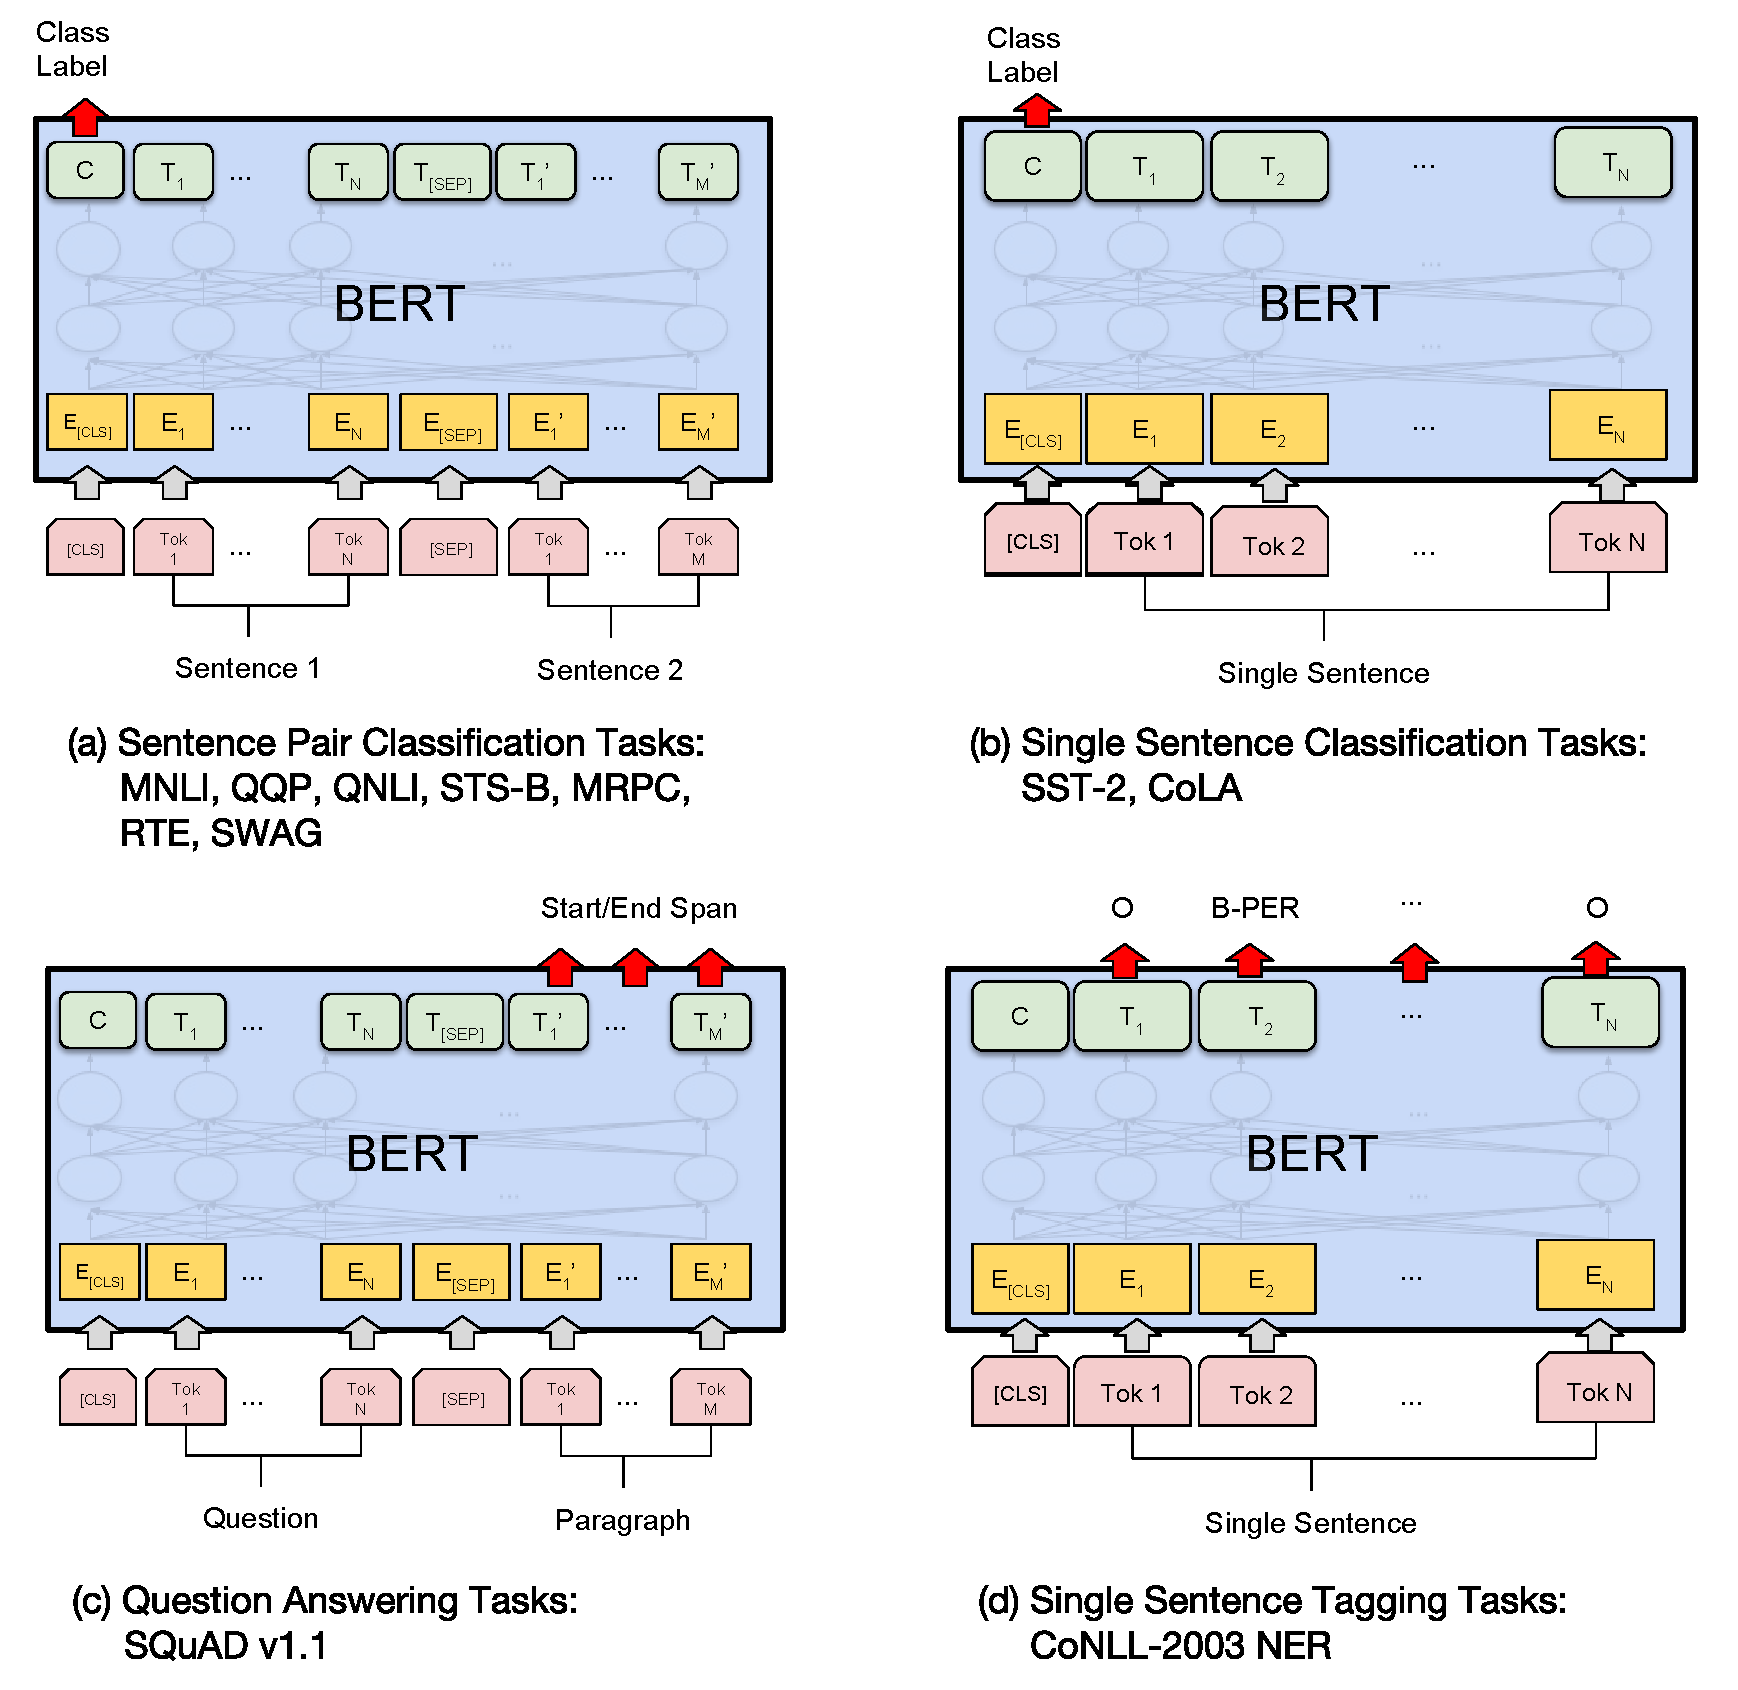
\includegraphics[width=0.85\textwidth]{BERT_fine_tune.pdf}
\end{center}
\caption{서로 다른 과제에 대한 BERT 파인튜닝 도식.}
\label{fig:bert_fine_tune}
\end{figure*}





%auto-ignore
\section{실험 세부 설정}
\label{appendix:sec:exp_details}

\subsection{GLUE 벤치마크 실험 상세 설명}
\label{appendix:sec:glue}

표~\ref{tab:glue_official}의 GLUE 결과는 \url{https://gluebenchmark.com/leaderboard}와 \url{https://blog.openai.com/language-unsupervised}에서 가져왔다.
GLUE 벤치마크는 다음 데이터셋들을 포함하며, 원래 \citet{wang-etal:2018:_glue}에 정리된 설명을 따른다.

\paragraph{MNLI} Multi-Genre Natural Language Inference는 크라우드소싱된 대규모 함의(entailment) 분류 과제다~\cite{williams-nangia-bowman:2018}. 한 쌍의 문장이 주어졌을 때, 두 번째 문장이 첫 번째 문장에 대해 \emph{함의}, \emph{모순}, \emph{중립} 중 어떤 관계인지를 예측하는 것이 목표다.

\paragraph{QQP} Quora Question Pairs는 Quora에 올라온 두 질문이 의미적으로 동일한지 판단하는 이진 분류 과제다~\cite{chen-etal:2018:_quora}.

\paragraph{QNLI} Question Natural Language Inference는 Stanford Question Answering Dataset~\cite{rajpurkar-etal:2016:_squad}을 이진 분류 과제로 변환한 버전이다~\cite{wang-etal:2018:_glue}. 양성 예시는 정답을 포함하는 (질문, 문장) 쌍이고, 음성 예시는 같은 단락에서 가져왔지만 답을 포함하지 않는 (질문, 문장) 쌍이다.

\paragraph{SST-2} Stanford Sentiment Treebank는 영화 리뷰에서 추출된 문장들에 사람의 감성 라벨이 붙은 단문장 이진 분류 과제다~\cite{socher-etal:2013:_recur}.

\paragraph{CoLA} Corpus of Linguistic Acceptability는 영어 문장이 언어학적으로 ``수용 가능''한지를 예측하는 단문장 이진 분류 과제다~\cite{warstadt-singh-bowman:2018:_corpus}.

\paragraph{STS-B} Semantic Textual Similarity Benchmark는 뉴스 헤드라인과 기타 출처에서 가져온 문장 쌍의 모음이다~\cite{cer-etal:2017}. 각 쌍에는 두 문장이 의미적으로 얼마나 유사한지를 1점에서 5점으로 표기한 라벨이 붙어 있다.

\paragraph{MRPC} Microsoft Research Paraphrase Corpus는 온라인 뉴스 출처에서 자동 추출된 문장 쌍에, 두 문장이 의미적으로 동일한지에 대한 사람 라벨이 붙은 데이터셋이다~\cite{dolan-brockett:2005:_autom}.

\paragraph{RTE} Recognizing Textual Entailment는 MNLI와 유사한 이진 함의 과제이지만 학습 데이터가 훨씬 적다~\cite{bentivogli-etal:2009}.\footnote{본 논문은 단일 과제 파인튜닝 결과만 보고한다. 다중 과제 파인튜닝은 성능을 더 끌어올릴 가능성이 있다 — 실제로 MNLI와의 다중 과제 학습이 RTE에서 큰 향상을 가져오는 것을 관찰했다.}

\paragraph{WNLI} Winograd NLI는 작은 자연어 추론 데이터셋이다~\cite{levesque-davis-morgenstern:2011:_winog}. GLUE 웹페이지는 이 데이터셋 구성에 문제가 있음을 지적하며,\footnote{\url{https://gluebenchmark.com/faq}} GLUE에 제출된 모든 학습 시스템이 다수 클래스를 예측하는 65.1\,\% 베이스라인 정확도보다 낮은 성능을 보였다. 따라서 OpenAI GPT와의 공정한 비교를 위해 본 데이터셋은 제외한다. 본 논문의 GLUE 제출에서는 항상 다수 클래스를 예측했다.




%auto-ignore

\section{추가 절제 연구}
\label{appendix:sec:more_ablation_studies}

\subsection{학습 스텝 수의 효과}
\label{sec:num_training_steps}

그림~\ref{fig:step_abalation}은 $k$ 스텝 동안 사전학습된 체크포인트에서 파인튜닝한 뒤의 MNLI Dev 정확도를 보여 준다. 이를 통해 다음 두 질문에 답할 수 있다.

%auto-ignore

\begin{figure}[b]
\begin{tikzpicture}
 \begin{axis}[
   width=0.95\columnwidth,
   height=0.7\columnwidth,
   legend cell align=left,
   legend style={at={(1, 0)},anchor=south east,font=\scriptsize},
   mark options={mark size=3},
   font=\scriptsize,
   xmin=0, xmax=1000,
   ymin=75, ymax=85,
   xtick={200,400,600,800,1000},
   ymajorgrids=true,
   xmajorgrids=true,
   xlabel style={yshift=0.5ex,},
   xlabel={사전학습 스텝 (천 단위)} ,
   ylabel={MNLI Dev 정확도},
   ylabel style={yshift=-0.5ex,}]
    \addplot[mark=triangle,g-blue] plot coordinates {
      (30, 78.6)
      (50, 79.6)
      (100, 80.5)
      (200, 82.2)
      (400, 83.2)
      (600, 84.0)
      (800, 84.3)
      (1000, 84.4)
    };
    \addlegendentry{\bertbase (Masked LM)}
    \addplot[mark=x,g-red] plot coordinates {
      (30, 79.4)
      (50, 79.8)
      (100, 80.3)
      (200, 81.0)
      (400, 81.7)
      (600, 81.9)
      (800, 82.1)
      (1000, 82.2)
    };
    \addlegendentry{\bertbase (Left-to-Right)}
     \end{axis}
\end{tikzpicture}
\caption{학습 스텝 수에 대한 절제. $k$ 스텝 동안 사전학습된 모델 파라미터에서 출발해 파인튜닝한 뒤의 MNLI 정확도를 보여 준다. x축은 $k$의 값이다.}
\label{fig:step_abalation}
\end{figure}

\begin{enumerate}
\item 질문: BERT가 높은 파인튜닝 정확도를 얻기 위해 정말로 그렇게 많은 사전학습(128,000 단어/배치 × 1,000,000 스텝)이 필요한가? \\
답: 그렇다. \bertbase는 500k 스텝 학습 대비 1M 스텝 학습 시 MNLI 정확도를 거의 1.0\,\% 더 얻는다.
\item 질문: 각 배치에서 모든 단어가 아닌 15\,\%만 예측하므로, MLM 사전학습이 LTR 사전학습보다 느리게 수렴하는가? \\
답: MLM 모델은 LTR 모델보다 약간 느리게 수렴한다. 그러나 절대 정확도 면에서, MLM 모델은 거의 즉시 LTR 모델을 능가하기 시작한다.
\end{enumerate}

\subsection{서로 다른 마스킹 절차에 대한 절제}
\label{appendix:sec:different_masks}

\S\ref{sec:pretraining_tasks}에서 언급했듯이, BERT는 마스킹 언어모델(MLM) 목적함수로 사전학습할 때 목표 토큰을 마스킹하는 데 혼합 전략을 쓴다. 다음은 서로 다른 마스킹 전략의 효과를 평가하는 절제 연구이다.

마스킹 전략의 목적은 사전학습과 파인튜닝 사이의 불일치를 줄이는 것임에 유의한다 — {\tt [MASK]} 기호가 파인튜닝 단계에는 등장하지 않기 때문이다. 저자들은 MNLI와 NER 양쪽의 Dev 결과를 보고한다. NER에 대해서는 파인튜닝 접근과 피처 기반 접근을 모두 보고하는데, 모델이 표현을 조정할 기회가 없는 피처 기반 접근에서는 불일치가 증폭될 것으로 예상되기 때문이다.

%auto-ignore
\begin{table}[ht]
\begin{center}
{\small
\begin{tabular}{@{}rrrccc@{}}
  \toprule
  \multicolumn{3}{c}{마스킹 비율} & \multicolumn{3}{c}{Dev 셋 결과} \\
  \cmidrule(r{0.2cm}){1-3}
  \cmidrule(l{0.2cm}){4-6}
  \textsc{Mask} &	\textsc{Same}&	\textsc{Rnd}	& {MNLI} &	\multicolumn{2}{c}{NER}\\
   &  & & {\footnotesize 파인튜닝} &   {\footnotesize 파인튜닝}	& {\footnotesize 피처 기반}\\
    \cmidrule(r{0.2cm}){1-3}
  \cmidrule(l{0.1cm}r{0.1cm}){4-4}
  \cmidrule(l{0.2cm}){5-6}
  
  80\%	&10\%	&10\%	&84.2	&95.4	&94.9\\
100\%	&0\%	&0\%	&84.3	&94.9	&94.0\\
80\%	&0\%	&20\%	&84.1	&95.2	&94.6\\
80\%	&20\%	&0\%	&84.4	&95.2	&94.7\\
0\%	&20\%	&80\%	&83.7	&94.8	&94.6 \\
0\%	&0\%	&100\%	&83.6	&94.9	&94.6\\
\bottomrule
\end{tabular}
} % small
\end{center}
\caption{\label{tab:mask_ablation} 서로 다른 마스킹 전략에 대한 절제.}
\end{table}



결과는 표~\ref{tab:mask_ablation}에 제시한다. 표에서 \textsc{Mask}는 MLM에서 목표 토큰을 {\tt [MASK]} 기호로 바꾸는 것을, \textsc{Same}은 목표 토큰을 그대로 두는 것을, \textsc{Rnd}는 목표 토큰을 다른 무작위 토큰으로 바꾸는 것을 의미한다.

표 왼쪽 부분의 숫자는 MLM 사전학습 동안 각 전략이 사용되는 확률을 나타낸다(BERT는 80\,\%, 10\,\%, 10\,\%를 사용). 오른쪽 부분은 Dev 셋 결과를 나타낸다. 피처 기반 접근에서는 \S\ref{sec:ner}에서 가장 좋은 방법으로 밝혀진, BERT의 마지막 4개 층을 결합한 피처를 사용한다.

표에서 보이듯, 파인튜닝은 서로 다른 마스킹 전략에 대해 놀라울 만큼 견고하다. 그러나 예상대로, 피처 기반 접근을 NER에 적용할 때 \textsc{Mask} 전략만 사용한 것은 문제가 있었다. 흥미롭게도, \textsc{Rnd} 전략만 사용한 것 역시 본 논문의 전략보다 훨씬 나쁜 성능을 보였다.










\end{document}
